% don't remove the folling lines, and edit the defintion of \main if needed
\documentclass[../report.tex]{subfiles}
\providecommand{\main}{..}
\IfEq{\jobname}{\currfilebase}{\AtEndDocument{\biblio}}{}
% until here

\begin{document}

\asection{Global effective field theory fits}\label{sec8:globalfit}
\label{sec8}

The absence to date of conclusive signals of physics beyond the Standard Model (SM) at the Large Hadron Collider (LHC) suggests
that there might be a separation of scales between the SM, and whatever may lie beyond it at some higher energy.
This motivates using the Standard Model Effective Field Theory (SMEFT) as a tool to search indirectly for new physics in LHC data,
given its (near) model-independence, capacity for systematic improvement, and ability to exploit simultaneously multiple datasets. For more motivation and details, see section~\ref{sec:eftintro}.
Beside the high-energy effects discussed in section \ref{sec4}, the HL and HE-LHC have a great potential in this context via the global fit to electroweak precision (EWPO) and Higgs
data, thanks to the higher precision they will reach both in the
measurement of some of the crucial input parameters of global EW fits
(e.g. $M_W$, $m_t$, $M_H$, and
$\sin^2\theta_{\mathrm{eff}}^{\mathrm{lept}}$) and the measurement
of Higgs-boson total rates.




This section focuses  on new physics effects, parametrised by extending
the SM Lagrangian via gauge-invariant dimension-six operators in \eq{EFTLAG} and estimates the reach on the Wilson coefficients provided by a global analysis, that is, an analysis with multiple observables and coefficients.
A global analysis of constraints on the Wilson coefficients of the SMEFT is of critical importance when more than a few coefficients are allowed to be non-zero,
since many SMEFT operators contribute to multiple observables, so that different classes of measurement should not be analysed in isolation.
The importance of this feature increases as
measurements from the LHC compete in precision with previous generation precision experiments.

Section~\ref{sec8:smeft} proposes a global fit  based on the ATLAS and CMS signal strength extrapolations from section~\ref{sec2:exp_combination} and on the use of Simplified Template Cross Sections (STXS) and estimates of the $WW$ production rate. Section~\ref{sec8:universalewpo} focuses on universal theories and exploits, instead of STXS, the information obtained in the analysis of high-energy observables in section~\ref{sec4}; moreover it includes projections of electroweak precision observables in the context of HL and HE LHC. Finally section~\ref{sec8:cubicetc} puts emphasis on the impact of a global fit on measurements of the Higgs cubic self-coupling at the HE LHC.

\label{sec8:intro}

\asubsection[J. Ellis, C.W. Murphy, V. Sanz, T. You]{Prospective SMEFT Constraints from HL- and HE-LHC Data}
\label{sec8:smeft}

In this note, after reviewing the SMEFT framework and our previous results~\cite{Ellis:2018gqa,Ellis:2014dva, Ellis:2014jta, Murphy:2017omb}, we present projections for the
prospective sensitivities of measurements with the approved High-Luminosity LHC (HL-LHC) project and the proposed High-Energy LHC (HE-LHC) project
to Wilson coefficients. 
Our projections are based on ATLAS and CMS estimates of the accuracies with which they
could measure Higgs production rates together with our estimates of the possible accuracies of STXS
measurements, assuming plausible future reductions in theoretical and systematic errors.


We focus on dimension-6 operators, and work to linear order in the Warsaw basis~\cite{Grzadkowski:2010es},
so as to make a consistent EFT expansion to order ${\cal O}(\Lambda^{-2})$. 
We choose $\alpha$, $G_F$, and $M_Z$ as input parameters for our computations, though we note that
the choice of input scheme does not have much impact on the results of a fit to Wilson coefficients if a sufficiently global analysis is performed~\cite{Brivio:2017bnu}.
There are 2499 baryon-number-preserving dimension-6 Wilson coefficients in the SMEFT~\cite{Alonso:2013hga}.
Here we assume a $U(3)^5$ flavor symmetry between the operator coefficients for the five lighter SM fermion fields,
which reduces the number of (real) coefficients to 76.
However only 20 of those parameters are relevant for the di-boson, electroweak precision and Higgs observables that we consider here.

In the Warsaw basis, the 11 operators from table \ref{tab:dim6ops} relevant for di-boson measurements and electroweak precision observables, 
whether through direct contributions or shifts in input parameters, can be written as~\footnote{The operator definitions and normalisations used here differ slightly from those used in the Warsaw basis in Ref.~\cite{Ellis:2018gqa}. For convenience we list here the relations between the Wilson coefficients in the two notations:
%
\begin{align*}
&\bar{C}_H = \frac{v^2}{\Lambda^2}C_6  \, , \,  \bar{C}_{H\ell}^{(3)} = \frac{v^2}{\Lambda^2} C_{HL}^{(3)}  \, , \, \bar{C}_{H\ell}^{(1)} = \frac{v^2}{\Lambda^2} C_{HL}  \, , \,  \bar{C}_{\ell\ell} = \frac{v^2}{\Lambda^2} C_{LL}  \, , \,  \bar{C}_{HD} = \frac{v^2}{\Lambda^2} C_{HD}  \, , \, \\ 
& \bar{C}_{HWB} = \frac{v^2}{\Lambda^2} g g^\prime C_{WB}  \, , \,  \bar{C}_{He,Hu,Hd} = \frac{v^2}{\Lambda^2} C_{He,Hu,Hd}  \, , \,  \bar{C}_{Hq}^{(3)} = \frac{v^2}{\Lambda^2} C_{HQ}^{(3)} \, , \, \bar{C}_{Hq}^{(1)} = \frac{v^2}{\Lambda^2} C_{HQ}  \, , \,  \\
& \bar{C}_W = \frac{v^2}{\Lambda^2} \frac{g}{3!} C_{3W} \, , \,  \bar{C}_{eH, dH, uH} = \frac{v^2}{\Lambda^2} C_{ye, yd, yu}  \, , \, \bar{C}_{H\square} = \frac{v^2}{\Lambda^2}  \frac{1}{2} C_H \, , \,  \bar{C}_{HW} = \frac{v^2}{\Lambda^2} g^2 C_{WW}  \, , \, \\
& \bar{C}_{HB} = \frac{v^2}{\Lambda^2} {g^\prime}^2 C_{BB}  \, , \, \bar{C}_{HG} = \frac{v^2}{\Lambda^2} g_s^2 C_{GG}  \, , \,  \bar{C}_G = \frac{v^2}{\Lambda^2} \frac{g_s}{3!} C_{3G}  \, .
\end{align*}
}  
%
{\small
\begin{align}
\label{eq8:L11}
\mathcal{L}_\text{SMEFT}^\text{Warsaw} &\supset \frac{C_{HL}^{(3)}}{\Lambda^2} (H^\dag i\overleftrightarrow{D}^I_\mu H)(\bar\ell \tau^I \gamma^\mu \ell) + \frac{C_{HL}}{\Lambda^2}(H^\dag i\overleftrightarrow{D}_\mu H)(\bar \ell \gamma^\mu \ell) +\frac{C_{LL}}{\Lambda^2}(\bar \ell \gamma_\mu \ell)(\bar \ell \gamma^\mu \ell) \nonumber \\
&+ \frac{C_{HD}}{\Lambda^2}\left|H^\dag D_\mu H\right|^2 + \frac{C_{WB}}{\Lambda^2} g g^\prime H^\dag \tau^I H\, W^I_{\mu\nu} B^{\mu\nu}  \nonumber  \\ 
&+ \frac{C_{He}}{\Lambda^2} (H^\dag i\overleftrightarrow{D}_\mu H)(\bar e \gamma^\mu e) \nonumber + \frac{C_{Hu}}{\Lambda^2} (H^\dag i\overleftrightarrow{D}_\mu H)(\bar u \gamma^\mu u) + \frac{C_{Hd}}{\Lambda^2} (H^\dag i\overleftrightarrow{D}_\mu H)(\bar d \gamma^\mu d) \nonumber \\
&+ \frac{C_{HQ}^{(3)}}{\Lambda^2} (H^\dag i\overleftrightarrow{D}^I_\mu H)(\bar q \tau^I \gamma^\mu q) + \frac{C_{HQ}}{\Lambda^2} (H^\dag i\overleftrightarrow{D}_\mu H)(\bar q \gamma^\mu q) + \frac{C_{3W}}{\Lambda^2} \frac{g}{3!} \epsilon^{IJK} W_\mu^{I\nu} W_\nu^{J\rho} W_\rho^{K\mu} \, ,
%in our original convention:
%\mathcal{L}_\text{SMEFT}^\text{Warsaw} &\supset \frac{\bar{C}_{H\ell}^{(3)}}{v^2} (H^\dag i\overleftrightarrow{D}^I_\mu H)(\bar\ell \tau^I \gamma^\mu \ell) + \frac{\bar{C}_{H\ell}^{(1)}}{v^2}(H^\dag i\overleftrightarrow{D}_\mu H)(\bar \ell \gamma^\mu \ell) +\frac{\bar{C}_{\ell\ell}}{v^2}(\bar \ell \gamma_\mu \ell)(\bar \ell \gamma^\mu \ell) \nonumber \\
%&+ \frac{\bar{C}_{HD}}{v^2}\left|H^\dag D_\mu H\right|^2 + \frac{\bar{C}_{HWB}}{v^2} H^\dag \tau^I H\, W^I_{\mu\nu} B^{\mu\nu}  \nonumber  \\ 
%&+ \frac{\bar{C}_{He}}{v^2} (H^\dag i\overleftrightarrow{D}_\mu H)(\bar e \gamma^\mu e) \nonumber + \frac{\bar{C}_{Hu}}{v^2} (H^\dag i\overleftrightarrow{D}_\mu H)(\bar u \gamma^\mu u) + \frac{\bar{C}_{Hd}}{v^2} (H^\dag i\overleftrightarrow{D}_\mu H)(\bar d \gamma^\mu d) \nonumber \\
%&+ \frac{\bar{C}_{Hq}^{(3)}}{v^2} (H^\dag i\overleftrightarrow{D}^I_\mu H)(\bar q \tau^I \gamma^\mu q) + \frac{\bar{C}_{Hq}^{(1)}}{v^2} (H^\dag i\overleftrightarrow{D}_\mu H)(\bar q \gamma^\mu q) + \frac{\bar{C}_{W}}{v^2} \epsilon^{IJK} W_\mu^{I\nu} W_\nu^{J\rho} W_\rho^{K\mu} \, ,
\end{align}
}
%
where Hermitian conjugate operators are implicit.
The flavor indices are trivial, except for the four-lepton operator, $C_{LL} = C_{\substack{LL \\ e\mu\mu e}} = C_{\substack{LL \\ \mu ee\mu}}$~\cite{Cirigliano:2009wk}, 
and are also left implicit.
There are an additional nine operators that contribute to Higgs measurements, 
%
{\small
\begin{align}
\label{eq8:L9}
\mathcal{L}_\text{SMEFT}^\text{Warsaw} &\supset  \frac{C_{y_e}}{\Lambda^2} y_e (H^\dag H)(\bar \ell e H) + \frac{C_{y_d}}{\Lambda^2} y_d (H^\dag H)(\bar q d H) + \frac{C_{y_u}}{\Lambda^2} y_u (H^\dag H)(\bar q u \widetilde H) \nonumber \\
&+ \frac{C_{3G}}{\Lambda^2} \frac{g_s}{3!} f^{ABC} G_\mu^{A\nu} G_\nu^{B\rho} G_\rho^{C\mu}  + \frac{C_{H}}{\Lambda^2} \frac{1}{2}\left(\partial^\mu |H|^2\right)^2  + \frac{C_{uG}}{\Lambda^2} y_u (\bar q \sigma^{\mu\nu} T^A u) \widetilde H \, G_{\mu\nu}^A   \nonumber \\
&+ \frac{C_{WW}}{\Lambda^2} g^2 H^\dag H\, W^I_{\mu\nu} W^{I\mu\nu} + \frac{C_{BB}}{\Lambda^2} {g^\prime}^2 H^\dag H\, B_{\mu\nu} B^{\mu\nu} + \frac{C_{GG}}{\Lambda^2} g_s^2 H^\dag H\, G^A_{\mu\nu} G^{A\mu\nu} \, .
%in our original convention:
%\mathcal{L}_\text{SMEFT}^\text{Warsaw} &\supset  \frac{\bar{C}_{eH}}{v^2} y_e (H^\dag H)(\bar \ell e H) + \frac{\bar{C}_{dH}}{v^2} y_d (H^\dag H)(\bar q d H) + \frac{\bar{C}_{uH}}{v^2} y_u (H^\dag H)(\bar q u \widetilde H) \nonumber \\
%&+ \frac{\bar{C}_{G}}{v^2} f^{ABC} G_\mu^{A\nu} G_\nu^{B\rho} G_\rho^{C\mu}  + \frac{\bar{C}_{H\Box}}{v^2} (H^\dag H)\Box(H^\dag H) + \frac{\bar{C}_{uG}}{v^2} y_u (\bar q \sigma^{\mu\nu} T^A u) \widetilde H \, G_{\mu\nu}^A   \nonumber \\
%&+ \frac{\bar{C}_{HW}}{v^2} H^\dag H\, W^I_{\mu\nu} W^{I\mu\nu} + \frac{\bar{C}_{HB}}{v^2}H^\dag H\, B_{\mu\nu} B^{\mu\nu} + \frac{\bar{C}_{HG}}{v^2} H^\dag H\, G^A_{\mu\nu} G^{A\mu\nu} \, .
\end{align}}
The explicit appearance of the Yukawa matrices in Eq.~\eqref{eq8:L9} is necessary to preserve formally the $U(3)^5$ flavor symmetry.
We neglect here $\mathcal{O}_6$ which is discussed in detail in sections \ref{sec3} and \ref{sec8:cubicetc}.
All of the operators in Eq.~\eqref{eq8:L11} except $\mathcal{O}_{3W}$ affect Higgs measurements at leading order, and
$\mathcal{O}_{3W}$ contributes to Higgs processes at next-to-leading order~\cite{Alonso:2013hga, Hartmann:2015oia, Hartmann:2015aia, Dedes:2018seb, Dawson:2018liq}.
We note also that Higgs production in association with a top-quark pair probes additional terms in the 
SMEFT~\cite{Maltoni:2016yxb, AguilarSaavedra:2018nen, Ellis:2018gqa} that do not contribute to the other observables we consider.
The only one we consider explicitly is $C_{uG}$, which makes the largest contribution to $t \bar{t} h$ production~\cite{Ellis:2018gqa}~\footnote{For 
an alternative analysis including all the operators, see~\cite{Murphy:2017omb}.}.

%\section{Fit Setup}
%\label{sec8:fit}
In our global fit to the current data we have used the predictions for electroweak precision observables and $WW$ scattering at LEP~2 in the 
Warsaw basis from Refs.~\cite{Berthier:2016tkq, Brivio:2017vri}, and predictions for LHC observables are made using $\mathtt{SMEFTsim}$~\cite{Brivio:2017btx}.
The following data are used in our global fit:

\begin{itemize}
\item \textit{Pre-LHC data}:  
We use 11 $Z$-pole observables from LEP 1 and one from SLC, as given in Ref.~\cite{ALEPH:2005ab}, as well as the $W$ mass measurement from the 
Tevatron~\cite{Aaltonen:2013iut}.
In addition, we use all the LEP~2 data for the processes $e^+ e^- \to W^+ W^- \to 4f$,
as compiled in Ref.~\cite{Berthier:2016tkq}, the original experimental papers being Refs.~\cite{Heister:2004wr, Achard:2004zw, Abbiendi:2007rs, Schael:2013ita}. 
These measurements probe eleven directions in the SMEFT, which can be mapped to the operators in Eq.~\eqref{eq8:L11}.

\item \textit{LHC Run 1 data}: 
We use all the 20 Higgs signal strengths from Table 8 of Ref.~\cite{Khachatryan:2016vau}.
We also use the ATLAS and CMS combination for the $h \to \mu^+ \mu^-$ signal strength~\cite{Khachatryan:2016vau}, and the ATLAS $h \to Z \gamma$ signal strength~\cite{Aad:2015gba}. 
We also include the $W$ mass measurement from ATLAS~\cite{Aaboud:2017svj}.

\item \textit{LHC Run 2 data}: 
We use 25 measurements from CMS~\cite{Sirunyan:2017dgc, Sirunyan:2017elk, Sirunyan:2018mvw, Sirunyan:2018shy, CMS-PAS-HIG-16-042, Sirunyan:2018ouh, Sirunyan:2017exp, Sirunyan:2017khh}, and 23 measurements from ATLAS~\cite{Aaboud:2017ojs, Aaboud:2017xsd, Aaboud:2017rss, Aaboud:2017jvq, ATLAS-CONF-2018-004, ATLAS-CONF-2017-047, ATLAS-CONF-2016-112}, including experimental correlations whenever possible. 
In addition, we include one ATLAS measurement at 13 \UTeV of the differential cross section for $p p \to W^+ W^- \to e^{\pm} \nu \mu^{\mp} \nu$
that requires $p_T > 120$~\UGeV for the leading lepton~\cite{Aaboud:2017qkn}.
\end{itemize}

\vspace{5mm}
\noindent
{\bf Selection of Current Results.} 
\label{sec8:curr}
In this Section we summarise the main result of the global fit to current data in Ref.~\cite{Ellis:2018gqa}. Fig.~\ref{fig8:HEPfitvsEMSY} summarises the sensitivities to operator coefficients in the Warsaw basis.
It shows the 95\% CL bounds in \UTeV on the Wilson coefficients, as obtained in~\cite{Ellis:2018gqa} from marginalised (orange) and individual (green) fits to the 20 dimension-6 operators 
entering in electroweak precision tests, di-boson and Higgs measurements at LEP, SLC, Tevatron, and LHC Runs 1 and 2.
Also shown, in blue, are the analogous results of the individual fits of the HEPfit Collaboration~\cite{Ciuchini:2013pca, deBlas:2016ojx}~\footnote{See 
also~\cite{luca:talk, otto:talk}. For a recent fit in another basis see Ref.~\cite{Alves:2018nof}, and
for a recent fit in the nonlinear Effective Theory see Ref.~\cite{deBlas:2018tjm}.}. 
We note that the degree of agreement in the individual operator fits is generally good. 


%%%%%%%
\begin{figure}
  \centering
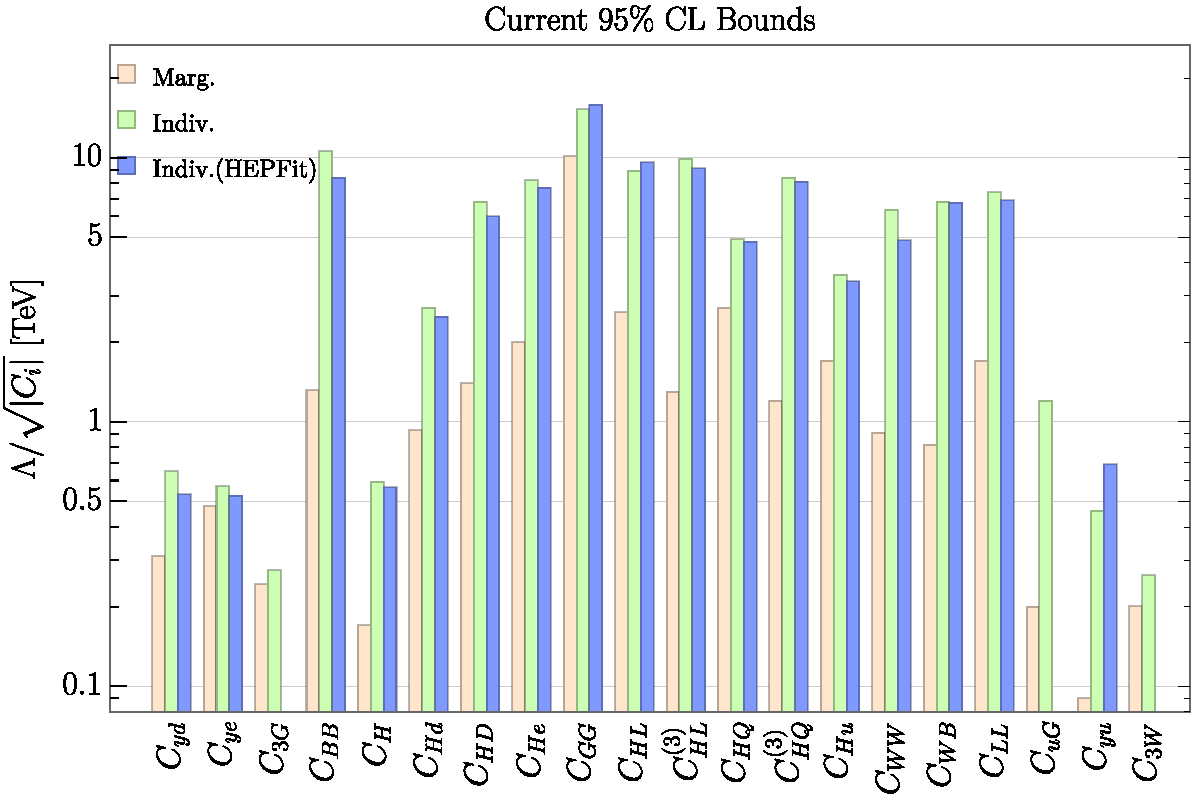
\includegraphics[width=0.8\textwidth]{section8/plots/barcompcnorm.pdf}
\vspace{-0.2cm}
 \caption{\it Current constraints on dimension-6 operators. The orange and green bars are the marginalised and individual limits from Ref.~\cite{Ellis:2018gqa}, respectively. 
 The analogous results of the HEPfit Collaboration~\cite{Ciuchini:2013pca, deBlas:2016ojx} for the case where only one operator is switched on at a time are shown in blue.}
   \label{fig8:HEPfitvsEMSY}
\end{figure} 

Table~\ref{tab8:FIpM} gives the Fisher information contained in a given dataset per number of measurements in that dataset,
for each coefficient in the case where one operator is switched on at a time.
The datasets are categorised as in Ref.~\cite{Ellis:2018gqa}, where a
cross indicates no (current) sensitivity.
This Table is the per-measurement analogue of Table 5 of Ref.~\cite{Ellis:2018gqa}, and
shows that LHC di-boson measurements are more powerful than LEP 2 di-boson measurements for constraining triple gauge couplings (TGCs).
In the Warsaw basis the three TGCs correspond to $C_{WB}$, $C_{3W}$, and a linear combination of $C_{HD}$, $C_{HL}^{(3)}$, $C_{WB}$, and $C_{LL}$.
We note, however, that $Z$-pole and Higgs-pole measurements are more constraining for all but $C_{3W}$. 

%%%%%%%
\begin{table}
\centering
 \begin{tabular}{|c|c|c|c|c|c|c|} \hline
Coefficient & $Z$-pole + $m_W$ & $WW$ at LEP2 & Higgs Run1 & Higgs Run2 & LHC $WW$ high-$p_T$  \\  \hline \hline
 $C_{yd}$ & $\times$ & $\times$ & 10 & 8.1 & $\times$  \\
 $C_{ye}$ & $\times$ & $\times$ & 2.9 & 1.3 & $\times$ \\
 $C_{3G}$ & $\times$ & $\times$ & 0.5 & 9.1 & $\times$  \\
 $C_{BB}$ & $\times$ & $\times$ & $9.9 \cdot 10^5$ & $2.0 \cdot 10^6$ & $\times$  \\
 $C_{H}$ & $\times$ & $\times$ & 8.1 & 15 & 0.1  \\
$C_{Hd}$ & $7.4 \cdot 10^3$ & $\times$ & 2.0 & 1.5 & 9.8  \\
 $C_{HD}$ & $4.3 \cdot 10^5$ & 51 & 4.6 & 4.5 & $5.5 \cdot 10^2$  \\
$C_{He}$ & $6.5 \cdot 10^5$ & 14 & $1.1 \cdot 10^{-2}$ & $3.7 \cdot 10^{-2}$ & $\times$  \\
 $C_{GG}$ & $\times$ & $\times$ & $9.8 \cdot 10^5$ & $8.6 \cdot 10^5$ & $1.5 \cdot 10^4$  \\
$C_{HL}$ & $1.1 \cdot 10^6$ & 51 & $1.1 \cdot 10^{-2}$ & $3.6 \cdot 10^{-2}$ & $4.6 \cdot 10^{-3}$  \\
 $C_{HL}^{(3)}$ & $1.7 \cdot 10^6$ & $1.3 \cdot 10^3$ & 51 & 49 & $3.5 \cdot 10^3$  \\
 $C_{HQ}$ & $6.4 \cdot 10^4$ & $\times$ & 2.3 & 1.0 & 37  \\
$C_{HQ}^{(3)}$ & $4.9 \cdot 10^5$ & $9.1 \cdot 10^2$ & $5.9 \cdot 10^2$ & $3.3 \cdot 10^2$ & $5.0 \cdot 10^3$  \\
 $C_{Hu}$ & $1.4 \cdot 10^4$ & $\times$ & 18 & 12 & 83  \\
$C_{WW}$ & $\times$ & $\times$ & $9.1 \cdot 10^4$ & $1.8 \cdot 10^5$ & $7.0 \cdot 10^{-3}$ \\
$C_{WB}$ & $3.3 \cdot 10^6$ & $1.9 \cdot 10^2$ & $3.0 \cdot 10^5$ & $5.7 \cdot 10^5$ & $2.2 \cdot 10^3$ \\
 $C_{LL}$ & $5.5 \cdot 10^5$ & $3.3 \cdot 10^2$ & 16 & 21 & $6.0 \cdot 10^2$ \\
$C_{uG}$ & $\times$ & $\times$ & 18 & 97 & $\times$  \\
 $C_{yu}$ & $\times$ & $\times$ & 0.4 & 1.8 & $\times$ \\
 $C_{3W}$ & $\times$ & 6.7 & $\times$ & $\times$ & 19 \\ \hline
 %original notation:
% $C_{dH}$ & $\times$ & $\times$ & 10 & 8.1 & $\times$  \\
% $C_{eH}$ & $\times$ & $\times$ & 2.9 & 1.3 & $\times$ \\
% $C_{G}$ & $\times$ & $\times$ & 0.5 & 9.1 & $\times$  \\
% $C_{HB}$ & $\times$ & $\times$ & $9.9 \cdot 10^5$ & $2.0 \cdot 10^6$ & $\times$  \\
% $C_{H\Box}$ & $\times$ & $\times$ & 8.1 & 15 & 0.1  \\
%$C_{Hd}$ & $7.4 \cdot 10^3$ & $\times$ & 2.0 & 1.5 & 9.8  \\
% $C_{HD}$ & $4.3 \cdot 10^5$ & 51 & 4.6 & 4.5 & $5.5 \cdot 10^2$  \\
%$C_{He}$ & $6.5 \cdot 10^5$ & 14 & $1.1 \cdot 10^{-2}$ & $3.7 \cdot 10^{-2}$ & $\times$  \\
% $C_{HG}$ & $\times$ & $\times$ & $9.8 \cdot 10^5$ & $8.6 \cdot 10^5$ & $1.5 \cdot 10^4$  \\
%$C_{H\ell}^{(1)}$ & $1.1 \cdot 10^6$ & 51 & $1.1 \cdot 10^{-2}$ & $3.6 \cdot 10^{-2}$ & $4.6 \cdot 10^{-3}$  \\
%% $C_{H\ell}^{(3)}$ & $1.7 \cdot 10^6$ & $1.3 \cdot 10^3$ & 51 & 49 & $3.5 \cdot 10^3$  \\
% $C_{Hq}^{(1)}$ & $6.4 \cdot 10^4$ & $\times$ & 2.3 & 1.0 & 37  \\
%$C_{Hq}^{(3)}$ & $4.9 \cdot 10^5$ & $9.1 \cdot 10^2$ & $5.9 \cdot 10^2$ & $3.3 \cdot 10^2$ & $5.0 \cdot 10^3$  \\
% $C_{Hu}$ & $1.4 \cdot 10^4$ & $\times$ & 18 & 12 & 83  \\
%$C_{HW}$ & $\times$ & $\times$ & $9.1 \cdot 10^4$ & $1.8 \cdot 10^5$ & $7.0 \cdot 10^{-3}$ \\
%$C_{HWB}$ & $3.3 \cdot 10^6$ & $1.9 \cdot 10^2$ & $3.0 \cdot 10^5$ & $5.7 \cdot 10^5$ & $2.2 \cdot 10^3$ \\
% $C_{\ell\ell}$ & $5.5 \cdot 10^5$ & $3.3 \cdot 10^2$ & 16 & 21 & $6.0 \cdot 10^2$ \\
%$C_{uG}$ & $\times$ & $\times$ & 18 & 97 & $\times$  \\
% $C_{uH}$ & $\times$ & $\times$ & 0.4 & 1.8 & $\times$ \\
% $C_{W}$ & $\times$ & 6.7 & $\times$ & $\times$ & 19 \\ \hline
\end{tabular}
\caption{\it Impacts of different sets of measurements on the fit to individual Wilson coefficients in the Warsaw basis as measured by the Fisher information contained in a given dataset per number of measurements in that dataset for each coefficient. A cross indicates no (current) sensitivity.}
\label{tab8:FIpM}
\end{table}
\vspace{5mm}

\noindent
{\bf Future Projections.}\label{sec8:proj}
We use the same framework as described in Ref.~\cite{Ellis:2018gqa} to project how the sensitivities to the Wilson coefficients of the SMEFT will change at HL- and HE-LHC. Our projection strategy is as follows:
we leave all pre-LHC, and LHC Run-1 measurements unchanged; we adopt the CMS and ATLAS WG2 recommendations for the HL- and HE-LHC sensitivities, using the HL-LHC S2 scenario for the experimental projections on the signal strength uncertainties and their associated correlation matrix (provided separately by ATLAS and CMS);
and the remaining statistical uncertainties at HL- and HE-LHC are assumed to scale naively with the integrated luminosities and cross sections:
\begin{equation}
\frac{\delta\mathcal{O}_{\text{HL}, i}}{\delta\mathcal{O}_{\text{today}, i}} = \sqrt{\frac{L_{\text{today}, i}}{L_{\text{HL}}}} \; , \;
\frac{\delta\mathcal{O}_{\text{HE}, i}}{\delta\mathcal{O}_{\text{today}, i}} = \sqrt{\frac{\sigma_{13, i}}{\sigma_{27, i}} \frac{L_{\text{today}, i}}{L_{\text{HE}}}}  . \nonumber
\end{equation}
For almost all the measurements by ATLAS(CMS) $L_{\text{today}, i} = 36.1(35.9)~\text{fb}^{-1}$,
and we use the benchmark luminosities $L_{\text{HL}} = 3~\text{ab}^{-1}$ and $L_{\text{HE}} = 15~\text{ab}^{-1}$ for all the measurements in the respective HL- and HE-LHC extrapolations.
The cross sections $\sigma_{13, i}$ and $\sigma_{27, i}$ refer to the SM cross sections in the signal region for a given measurement $i$ at 13 and 27 \UTeV, respectively. At HE-LHC the S2 systematics are reduced by half. For the STXS and $WW$ measurements used in Ref.~\cite{Ellis:2018gqa}, since no official projections have been made yet, we extrapolate the statistical part as described above and treat the systematics as unchanged for HL-LHC and halve them for HE-LHC. The correlations between experimental measurements are assumed to be unchanged.

We stress that both our projection scenarios are pessimistic in the sense that they do not take into account the additional channels~\cite{gilbert:talk}, finer binning~\cite{deFlorian:2016spz, Hays:2290628, ATLAS-CONF-2017-047} and extension of the STXS method to larger kinematic regions that will become available as more data are collected.
Furthermore, as suggested by Table~\ref{tab8:FIpM}, our projections under-utilise LHC di-boson scattering measurements~\cite{Azatov:2017kzw, Franceschini:2017xkh, Dawson:2018dcd}. 

\begin{figure}
  \centering
 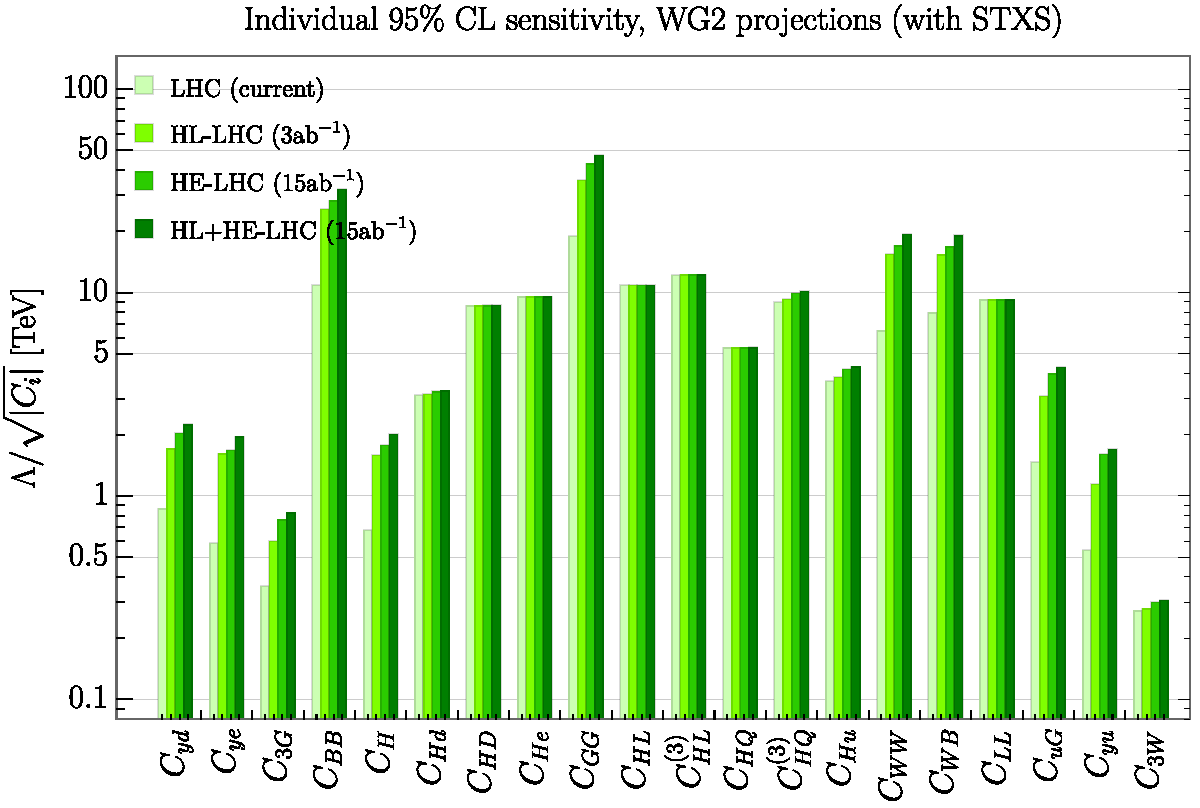
\includegraphics[width=0.8\textwidth]{section8/plots/individualbarchart.pdf}
 \vspace{-0.2cm}
 \caption{\it Individual 95\% CL projected sensitivities for LHC, HL-LHC, HE-LHC, and combined HL/HE-LHC in increasingly darker shades of green. The vertical axis gives the reach to the scale of new physics divided by the dimensionless Wilson coefficient, in units of \UTeV. }
   \label{fig:indiv}
\end{figure} 

\begin{figure}
  \centering
 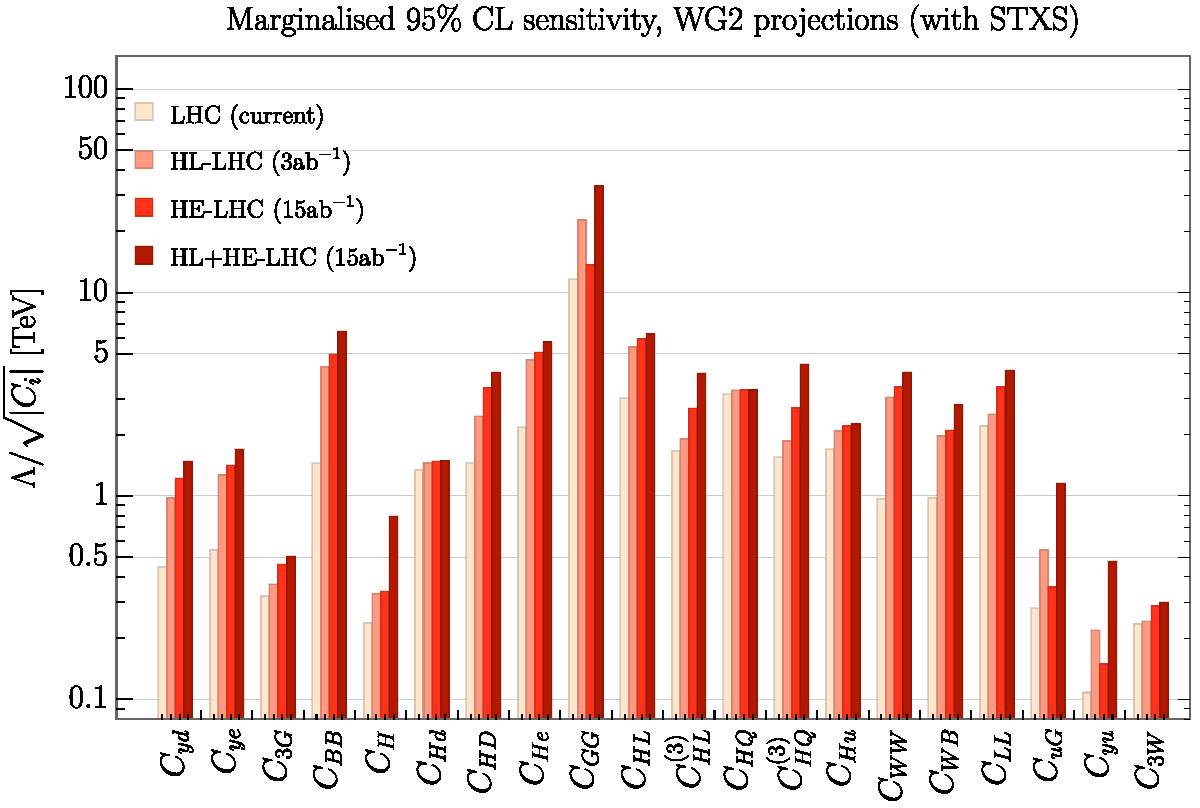
\includegraphics[width=0.8\textwidth]{section8/plots/marginalisedbarchart.pdf}
 \vspace{-0.2cm}
 \caption{\it  Marginalised 95\% CL projected sensitivities for LHC, HL-LHC, HE-LHC, and combined HL/HE-LHC in increasingly darker shades of red. The vertical axis gives the reach to the scale of new physics divided by the dimensionless Wilson coefficient, in units of \UTeV.}
   \label{fig:marg}
\end{figure} 

The results of our projections are shown in Figures~\ref{fig:indiv} and~\ref{fig:marg} for individual and marginalised 95\% CL sensitivities respectively. The vertical axis is the operator scale in units of \UTeV divided by the square root of the dimensionless Wilson coefficient. Increasingly darker shades for the four bars represent the sensitivities of the LHC up to now, HL-LHC with 3 ab$^{-1}$, HE-LHC with 15 ab$^{-1}$, and combining HL- and HE-LHC results (neglecting any correlations between the two). We see that in the individual bounds the sensitivity for each operator increases correspondingly, except for those that are only constrained by electroweak precision tests, which remain unchanged from their current LEP limits. In the marginalised case even the latter operators benefit from an improvement in the limits on other operators. We note that in going from HL- to HE-LHC there is a decrease in the marginalised sensitivity for $C_{GG}, C_{uG}$, and $C_{yu}$, despite improvements in their individual bounds. This is because $C_{uG}$ and $C_{yu}$ enter only in $tth$ production, and the relative increase in their contribution with respect to $C_{GG}$ in going from 13 to 27 \UTeV opens up a relatively flat direction in the parameter space, reducing the sensitivity to all three coefficients. This degeneracy can be broken by measurements at different energies, as shown in the combined HL/HE-LHC fit, or by including measurements involving top quarks.

In general, we see that data from HL- and/or HE-LHC would extend the sensitivity to new physics into the multi-\UTeV range
for most operator coefficients, extending to tens of \UTeV for $C_{GG}$.



%%%%%%%%%%%%%%%%%%%%%%
%\subsubsection*{Acknowledgements}
%The work of JE is supported partly by the United Kingdom STFC Grant ST/P000258/1 and partly by the Estonian Research Council via a Mobilitas Pluss grant. VS acknowledges support from the STFC Grant ST/P000819/1. The work of CM was partially supported by the United States Department of Energy under Grant Contract DE-SC0012704. The work of TY is supported by a Branco Weiss Society in Science Fellowship and a Junior Research Fellowship from Gonville and Caius College and partially supported by STFC Grant ST/P000681/1.






\subfile{\main/section8/hepfit_EFTfit.tex}



\FloatBarrier
\subfile{\main/section8/selfcoupling.tex}



\end{document}
